\section{Introduction}

In our work we use the Neurorobotics Platform (NRP). The NRP is a web platform that offers the ability to simulate robots in complex environments making use of a physics engine to simulate gravity, inertia, etc. The platform uses ROS to interface with the robot models, making a transfer to the real robots easier.

The aim of the work was to get a robot arm model to throw a cylinder model as far as possible inside the simulation environment. Both the robot arm and the cylinder are on top of a table.

The robot arm and the cylinder are shown in figure \ref{fig:challenge}.

\begin{figure}
	\begin{center}
		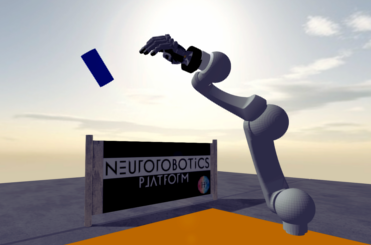
\includegraphics[width=0.4\textwidth]{hbpprak_2018}
	\end{center}
	\caption{The robot arm throwing the cylinder away from the table.}
	\label{fig:challenge}
\end{figure}

This submission report is structured as follows: section \ref{sec:motivation} motivates our choice of algorithms for solving the  Praktikum challenge. Sections \ref{sec:EA} and \ref{sec:MCMC} describe these algorithms in general. Sections \ref{sec:PrepareHit}, \ref{sec:Throw}, and \ref{sec:Windup} describe our approaches for solving the challenge.
Section \ref{sec:problems} discusses problems which occured during implementation and execution of these approaches. Finally, section \ref{sec:conclusion} summarizes the approaches and draws a conclusion.
